\documentclass[coverwidth=148mm, coverheight=210mm, spinewidth=37mm,
flapwidth=7cm, wrapwidth=3mm, 11pt]{bookcover}

\usepackage[utf8]{inputenc}
\usepackage[spanish,es-tabla]{babel}
\usepackage{microtype}
\usepackage{qrcode}
\usepackage[outline]{contour}
\contourlength{.5pt}

\usepackage[sc]{mathpazo} % Use the Palatino font with smallcaps
%\usepackage[osf]{mathpazo} % Palatino with smallcaps and oldstyle numbers

% \usepackage{avant} % Avant Garde Sans Serif
% \usepackage{helvet}
%\usepackage{tgadventor}
%\usepackage{AlegreyaSans}
\usepackage{biolinum}
%\usepackage{fetamont}
\usepackage{eulervm} % Euler math


\usepackage[T1]{fontenc}
\usepackage{microtype}

\definecolor{openscadyellow}{HTML}{FFFFE5}

\newbookcovercomponenttype{center rotate}{
  \vfill
  \centering
  \rotatebox[origin=c]{90}{#1}
  \vfill}

\newbookcovercomponenttype{rotate}{
  \centering
  \rotatebox[origin=c]{90}{#1}%
}

\begin{document}

\begin{bookcover}

  \begin{bookcoverelement}{color}{bg whole}
    openscadyellow
  \end{bookcoverelement}

  \begin{bookcoverelement}{center}{front}
    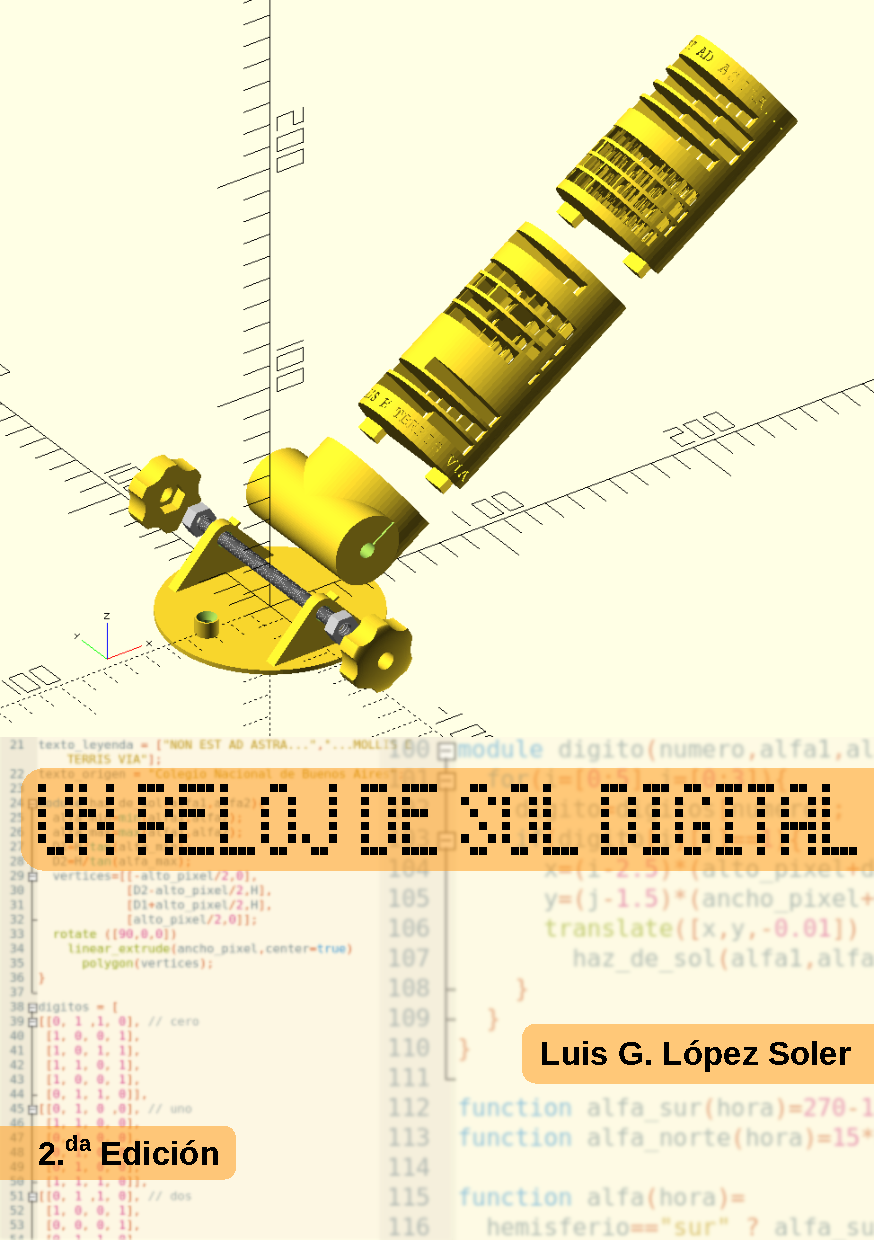
\includegraphics[width=\partwidth]{tapa-A5.pdf}
  \end{bookcoverelement}

  \begin{bookcoverelement}{center}{back}
    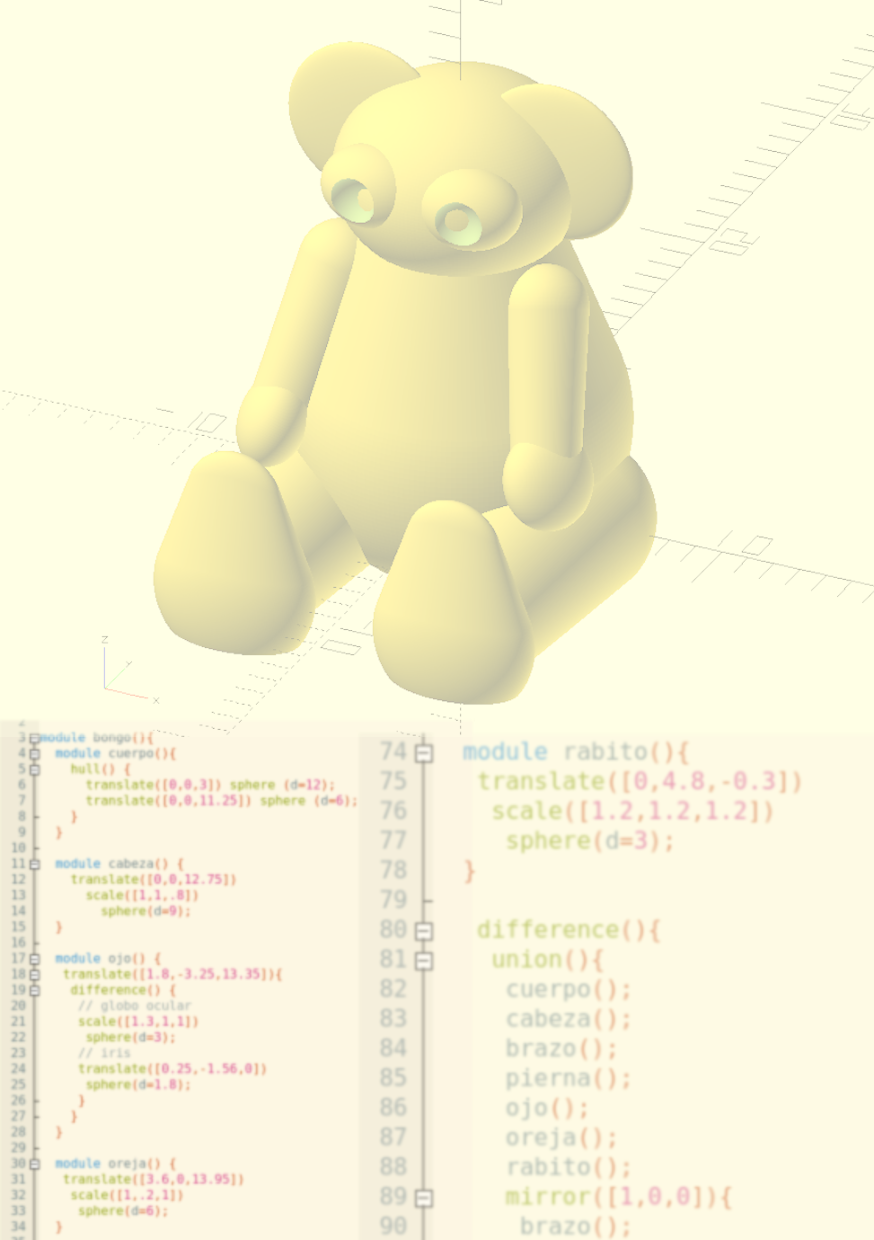
\includegraphics{contratapa-A5.pdf}
  \end{bookcoverelement}


  \begin{bookcoverelement}{normal}{back}[1.5cm,2cm,2cm,1cm]
    {\large

      \hspace{.5em} [...] Cecilia pensó que Antonia tenía razón. El objeto
      que tenía entre sus manos y que volvía y revolvía en ellas era muy
      hermoso; tanto más que aún no lo comprendía del todo y por lo
      tanto estaba cargado con todas las promesas del misterio y las
      posibilidades de la geometría. <<Este objeto>> ---pensó
      Cecilia--- <<será infinito mientras no lo comprenda del
      todo>>. No obstante, sabía que la pulsión por entender la
      vencería, y la finitud se cerniría sobre ese semicilindro de
      plástico que sus dedos acariciaban.

      \hspace{.5em} ---¿No me vas a preguntar cómo lo hice? ---Antonia
      hizo pucherito, simulando contrariedad y sonriendo con los ojos.

      \hspace{.5em} Cecilia salió con una sonrisa de su
      ensimismamiento y se dispuso a escuchar. [...]
  

  \begin{flushright}
    \emph{Fragmento del capítulo 3}
  \end{flushright}

  \vspace{2.5em}
  
  \hspace{.5em} [...] ---No parece un problema muy difícil de resolver
  ---a\-ven\-tu\-ró Cecilia---; supongo que deberemos escribir dos
  relaciones matemáticas entre horas y ángulos: una para cada
  hemisferio. Y permitir que el usuario indique, mediante una
  variable, si desea usar su reloj en el norte o en el sur, y en
  función de eso emplear una u otra relación: suena a una tarea para
  un \texttt{if}.

  \hspace{.5em} Antonia sonreía mientras escuchaba y caminaba junto a
  Cecilia. Pensó que ya empezaba a sonar como una programadora:
  elevando suposiciones al rango de algoritmos, cifrando sentencias
  breves al borde de lo confuso, y hasta enfrentando problemas aún no
  resueltos con una confianza demasiado parecida a la pedantería. Por
  un momento temió estar echándola a perder; pero decidió que, en
  cualquier caso, ya era demasiado tarde. [...]

  \begin{flushright}
    \emph{Fragmento del capítulo 23}
  \end{flushright}
}
  
  \end{bookcoverelement}

  \begin{bookcoverelement}{normal}{front flap}[1cm,2cm,1cm,1cm]

    \begin{center}
      \vspace{2cm}
      [Falta foto]
      \vspace{2cm}
%      \includegraphics[width=.75\partwidth]{[Foto]}
    \end{center}

    \bigskip
    
    \color{black} Luis Gabriel López Soler nació en Buenos Aires en
    diciembre de 1971.

    \hspace{.5em} Si bien el sistema educativo de su país asegura que
    es profesor de música, él se autopercibe profesor de astronomía;
    percepción ésta que las autoridades del Colegio Nacional de Buenos
    Aires, en cuyo Observatorio se desempeña como docente desde hace
    más de 25 años, parecen compartir o al menos tolerar.

    \hspace{.5em} Su mayor congoja consiste en no ser
    matemático, y su único orgullo no haber recibido, jamás, ningún
    premio. La flecha del tiempo parece asegurar ya, inexorable, la
    perfecta consecución de ambos accidentes.

    \hspace{.5em} La programación es uno de sus géneros literarios
    preferidos.

  \end{bookcoverelement}

  \begin{bookcoverelement}{normal}{back flap}[1cm,1cm,1cm,1cm]

        El presente libro fue compuesto con \LaTeX; su código fuente
    completo se encuentra aquí:

    \begin{center}
      \colorbox{white}{%
        \qrcode[height=2.5cm]{https://github.com/lopezsolerluis/reloj-de-sol-libro}}
    \end{center}

    \bigskip
    
    El código fuente del reloj de Sol digital puede obtenerse aquí:

    \begin{center}
      \colorbox{white}{%
        \qrcode[height=2.5cm]{https://github.com/lopezsolerluis/reloj-de-sol-digital}}
    \end{center}

    
    \vfill


    
\includegraphics[height=1.7em]{../cc-88x31} Esta obra está ba\-jo una
    licencia \emph{Creative Commons Atribución-CompartirIgual 4.0
      Internacional}.

    \begin{center}
      \colorbox{white}{%
        \qrcode[height=2.5cm]{http://creativecommons.org/licenses/by-sa/4.0/}}
    \end{center}


  \end{bookcoverelement}
  
  \begin{bookcoverelement}{rotate}{spine}
    \color{orange!70!white}

   \LARGE\sffamily\bfseries
   \contour{black}{Luis G. López Soler}
   \hspace{.03\partheight}

  \end{bookcoverelement}
  

  \begin{bookcoverelement}{rotate}{spine}
    \color{orange!70!white}%
    \fontsize{32}{40}\selectfont\sffamily\bfseries%
    \contour{black}{Un reloj de Sol digital}%
    \hspace{.42\partheight}    
  \end{bookcoverelement}

\end{bookcover}

\end{document}
